\PassOptionsToPackage{unicode=true}{hyperref} % options for packages loaded elsewhere
\PassOptionsToPackage{hyphens}{url}
%
\documentclass[]{ctexart}
\usepackage{lmodern}
\usepackage{amssymb,amsmath}
\usepackage{ifxetex,ifluatex}
\usepackage{fixltx2e} % provides \textsubscript
\ifnum 0\ifxetex 1\fi\ifluatex 1\fi=0 % if pdftex
  \usepackage[T1]{fontenc}
  \usepackage[utf8]{inputenc}
  \usepackage{textcomp} % provides euro and other symbols
\else % if luatex or xelatex
  \usepackage{unicode-math}
  \defaultfontfeatures{Ligatures=TeX,Scale=MatchLowercase}
    \setmonofont[Mapping=tex-ansi]{Fira Mono}
\fi
% use upquote if available, for straight quotes in verbatim environments
\IfFileExists{upquote.sty}{\usepackage{upquote}}{}
% use microtype if available
\IfFileExists{microtype.sty}{%
\usepackage[]{microtype}
\UseMicrotypeSet[protrusion]{basicmath} % disable protrusion for tt fonts
}{}
\IfFileExists{parskip.sty}{%
\usepackage{parskip}
}{% else
\setlength{\parindent}{0pt}
\setlength{\parskip}{6pt plus 2pt minus 1pt}
}
\usepackage{hyperref}
\hypersetup{
            pdftitle={Exploratory Data Analysis},
            pdfborder={0 0 0},
            breaklinks=true}
\urlstyle{same}  % don't use monospace font for urls
\usepackage[left=2cm, right=2cm, top=2.5cm, bottom=2.5cm]{geometry}
\usepackage{color}
\usepackage{fancyvrb}
\newcommand{\VerbBar}{|}
\newcommand{\VERB}{\Verb[commandchars=\\\{\}]}
\DefineVerbatimEnvironment{Highlighting}{Verbatim}{commandchars=\\\{\}}
% Add ',fontsize=\small' for more characters per line
\usepackage{framed}
\definecolor{shadecolor}{RGB}{248,248,248}
\newenvironment{Shaded}{\begin{snugshade}}{\end{snugshade}}
\newcommand{\AlertTok}[1]{\textcolor[rgb]{0.94,0.16,0.16}{#1}}
\newcommand{\AnnotationTok}[1]{\textcolor[rgb]{0.56,0.35,0.01}{\textbf{\textit{#1}}}}
\newcommand{\AttributeTok}[1]{\textcolor[rgb]{0.77,0.63,0.00}{#1}}
\newcommand{\BaseNTok}[1]{\textcolor[rgb]{0.00,0.00,0.81}{#1}}
\newcommand{\BuiltInTok}[1]{#1}
\newcommand{\CharTok}[1]{\textcolor[rgb]{0.31,0.60,0.02}{#1}}
\newcommand{\CommentTok}[1]{\textcolor[rgb]{0.56,0.35,0.01}{\textit{#1}}}
\newcommand{\CommentVarTok}[1]{\textcolor[rgb]{0.56,0.35,0.01}{\textbf{\textit{#1}}}}
\newcommand{\ConstantTok}[1]{\textcolor[rgb]{0.00,0.00,0.00}{#1}}
\newcommand{\ControlFlowTok}[1]{\textcolor[rgb]{0.13,0.29,0.53}{\textbf{#1}}}
\newcommand{\DataTypeTok}[1]{\textcolor[rgb]{0.13,0.29,0.53}{#1}}
\newcommand{\DecValTok}[1]{\textcolor[rgb]{0.00,0.00,0.81}{#1}}
\newcommand{\DocumentationTok}[1]{\textcolor[rgb]{0.56,0.35,0.01}{\textbf{\textit{#1}}}}
\newcommand{\ErrorTok}[1]{\textcolor[rgb]{0.64,0.00,0.00}{\textbf{#1}}}
\newcommand{\ExtensionTok}[1]{#1}
\newcommand{\FloatTok}[1]{\textcolor[rgb]{0.00,0.00,0.81}{#1}}
\newcommand{\FunctionTok}[1]{\textcolor[rgb]{0.00,0.00,0.00}{#1}}
\newcommand{\ImportTok}[1]{#1}
\newcommand{\InformationTok}[1]{\textcolor[rgb]{0.56,0.35,0.01}{\textbf{\textit{#1}}}}
\newcommand{\KeywordTok}[1]{\textcolor[rgb]{0.13,0.29,0.53}{\textbf{#1}}}
\newcommand{\NormalTok}[1]{#1}
\newcommand{\OperatorTok}[1]{\textcolor[rgb]{0.81,0.36,0.00}{\textbf{#1}}}
\newcommand{\OtherTok}[1]{\textcolor[rgb]{0.56,0.35,0.01}{#1}}
\newcommand{\PreprocessorTok}[1]{\textcolor[rgb]{0.56,0.35,0.01}{\textit{#1}}}
\newcommand{\RegionMarkerTok}[1]{#1}
\newcommand{\SpecialCharTok}[1]{\textcolor[rgb]{0.00,0.00,0.00}{#1}}
\newcommand{\SpecialStringTok}[1]{\textcolor[rgb]{0.31,0.60,0.02}{#1}}
\newcommand{\StringTok}[1]{\textcolor[rgb]{0.31,0.60,0.02}{#1}}
\newcommand{\VariableTok}[1]{\textcolor[rgb]{0.00,0.00,0.00}{#1}}
\newcommand{\VerbatimStringTok}[1]{\textcolor[rgb]{0.31,0.60,0.02}{#1}}
\newcommand{\WarningTok}[1]{\textcolor[rgb]{0.56,0.35,0.01}{\textbf{\textit{#1}}}}
\usepackage{graphicx,grffile}
\makeatletter
\def\maxwidth{\ifdim\Gin@nat@width>\linewidth\linewidth\else\Gin@nat@width\fi}
\def\maxheight{\ifdim\Gin@nat@height>\textheight\textheight\else\Gin@nat@height\fi}
\makeatother
% Scale images if necessary, so that they will not overflow the page
% margins by default, and it is still possible to overwrite the defaults
% using explicit options in \includegraphics[width, height, ...]{}
\setkeys{Gin}{width=\maxwidth,height=\maxheight,keepaspectratio}
\setlength{\emergencystretch}{3em}  % prevent overfull lines
\providecommand{\tightlist}{%
  \setlength{\itemsep}{0pt}\setlength{\parskip}{0pt}}
\setcounter{secnumdepth}{5}
% Redefines (sub)paragraphs to behave more like sections
\ifx\paragraph\undefined\else
\let\oldparagraph\paragraph
\renewcommand{\paragraph}[1]{\oldparagraph{#1}\mbox{}}
\fi
\ifx\subparagraph\undefined\else
\let\oldsubparagraph\subparagraph
\renewcommand{\subparagraph}[1]{\oldsubparagraph{#1}\mbox{}}
\fi

% set default figure placement to htbp
\makeatletter
\def\fps@figure{htbp}
\makeatother

\let\oldhref\href
\renewcommand{\href}[2]{\oldhref{#1}{\textcolor{blue}{\underline{#2}}}}

\let\oldhyperlink\hyperlink
\renewcommand{\hyperlink}[2]{\oldhyperlink{#1}{\textcolor{red}{\underline{#2}}}}
\usepackage{etoolbox}
\makeatletter
\providecommand{\subtitle}[1]{% add subtitle to \maketitle
  \apptocmd{\@title}{\par {\large #1 \par}}{}{}
}
\makeatother

\title{Exploratory Data Analysis}
\providecommand{\subtitle}[1]{}
\subtitle{可重复性报告 - 作为报告草稿}
\author{}
\date{\vspace{-2.5em}}

\begin{document}
\maketitle

{
\setcounter{tocdepth}{2}
\tableofcontents
}
\hypertarget{ux73afux5883}{%
\section{环境}\label{ux73afux5883}}

\hypertarget{r-info}{%
\subsection{R info}\label{r-info}}

\begin{Shaded}
\begin{Highlighting}[]
\NormalTok{xfun}\OperatorTok{::}\KeywordTok{session_info}\NormalTok{(}
        \DataTypeTok{packages =} \KeywordTok{c}\NormalTok{(}
                \StringTok{"readr"}\NormalTok{, }\StringTok{"tidyr"}\NormalTok{, }\StringTok{"stringr"}\NormalTok{, }\StringTok{"dplyr"}\NormalTok{, }\StringTok{"purrr"}\NormalTok{,}
                \StringTok{"ggplot2"}\NormalTok{, }\StringTok{"lubridate"}\NormalTok{, }\StringTok{"ggdag"}\NormalTok{, }\StringTok{"showtext"}
\NormalTok{        ), }\DataTypeTok{dependencies =} \OtherTok{FALSE}
\NormalTok{)}
\end{Highlighting}
\end{Shaded}

\begin{verbatim}
R version 4.1.0 (2021-05-18)
Platform: x86_64-pc-linux-gnu (64-bit)
Running under: Ubuntu 20.04.2 LTS

Locale:
  LC_CTYPE=zh_CN.UTF-8       LC_NUMERIC=C              
  LC_TIME=zh_CN.UTF-8        LC_COLLATE=zh_CN.UTF-8    
  LC_MONETARY=zh_CN.UTF-8    LC_MESSAGES=zh_CN.UTF-8   
  LC_PAPER=zh_CN.UTF-8       LC_NAME=C                 
  LC_ADDRESS=C               LC_TELEPHONE=C            
  LC_MEASUREMENT=zh_CN.UTF-8 LC_IDENTIFICATION=C       

Package version:
  dplyr_1.0.6      ggdag_0.2.3      ggplot2_3.3.3    lubridate_1.7.10
  purrr_0.3.4      readr_1.4.0      showtext_0.9-2   stringr_1.4.0   
  tidyr_1.1.3     
\end{verbatim}

\hypertarget{python-info}{%
\subsection{python info}\label{python-info}}

// TODO

\hypertarget{ux5206ux6790}{%
\section{分析}\label{ux5206ux6790}}

\hypertarget{the-workflow}{%
\subsection{The Workflow}\label{the-workflow}}

\begin{figure}
\centering
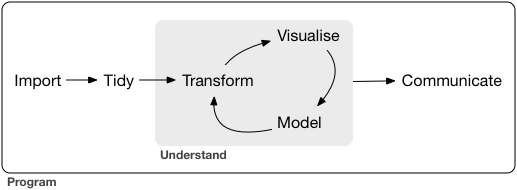
\includegraphics{workflow.png}
\caption[The Data Science Workflow]{The Data Science
Workflow\footnotemark{}}
\end{figure}
\footnotetext{This picture is from
  \href{https://r4ds.had.co.nz/introduction.html}{R for Data Science} by
  Hadley Wickham and Garrett Grolemund, released under
  \href{http://creativecommons.org/licenses/by-nc-nd/3.0/us/}{CC
  BY-NC-ND 3.0 US}.}

\hypertarget{import}{%
\subsection{Import}\label{import}}

// 需要数据集的完整描述和获取方式

// TODO - \textbf{R. Li}

\hypertarget{tidy}{%
\subsection{Tidy}\label{tidy}}

\begin{Shaded}
\begin{Highlighting}[]
\NormalTok{raw_df <-}\StringTok{ }\KeywordTok{read_csv}\NormalTok{(}\StringTok{"./data/investment/FDI_untidy.csv"}\NormalTok{)}

\NormalTok{process <-}\StringTok{ }\ControlFlowTok{function}\NormalTok{(raw_df) \{}
\NormalTok{  simplified_df <-}\StringTok{ }\NormalTok{raw_df }\OperatorTok
\StringTok{    }\KeywordTok{filter}\NormalTok{(X1 }\OperatorTok\StringTok{ }\KeywordTok{str_detect}\NormalTok{(}\StringTok{"^}\CharTok{\textbackslash{}\textbackslash{}}\StringTok{d"}\NormalTok{)) }\OperatorTok
\StringTok{    }\KeywordTok{rename}\NormalTok{(时间 =}\StringTok{ }\NormalTok{X1)}

\NormalTok{  fliped_df <-}\StringTok{ }\NormalTok{simplified_df }\OperatorTok
\StringTok{    }\KeywordTok{pivot_longer}\NormalTok{(}\KeywordTok{c}\NormalTok{(}\OperatorTok{-}\NormalTok{时间), }\DataTypeTok{names_to =} \StringTok{"observation"}\NormalTok{, }\DataTypeTok{values_to =} \StringTok{"val"}\NormalTok{)}

\NormalTok{  stdize <-}\StringTok{ }\ControlFlowTok{function}\NormalTok{(str) \{}
\NormalTok{    str }\OperatorTok
\StringTok{      }\KeywordTok{str_replace}\NormalTok{(}\DataTypeTok{pattern =} \StringTok{"(.*):(总计|一带一路)"}\NormalTok{, }\DataTypeTok{replacement =} \StringTok{"}\CharTok{\textbackslash{}\textbackslash{}}\StringTok{1/}\CharTok{\textbackslash{}\textbackslash{}}\StringTok{2/}\CharTok{\textbackslash{}\textbackslash{}}\StringTok{2"}\NormalTok{) }\OperatorTok
\StringTok{      }\KeywordTok{str_replace}\NormalTok{(}\DataTypeTok{pattern =} \StringTok{"::"}\NormalTok{, }\DataTypeTok{replacement =} \StringTok{":"}\NormalTok{) }\OperatorTok
\StringTok{      }\KeywordTok{str_replace}\NormalTok{(}\DataTypeTok{pattern =} \StringTok{"(.*):(.*洲):*(.*)"}\NormalTok{, }\DataTypeTok{replacement =} \StringTok{"}\CharTok{\textbackslash{}\textbackslash{}}\StringTok{1/}\CharTok{\textbackslash{}\textbackslash{}}\StringTok{2/}\CharTok{\textbackslash{}\textbackslash{}}\StringTok{3"}\NormalTok{)}
\NormalTok{  \}}

\NormalTok{  sep_df <-}\StringTok{ }\NormalTok{fliped_df }\OperatorTok
\StringTok{    }\KeywordTok{mutate}\NormalTok{(}\DataTypeTok{observation =}\NormalTok{ observation }\OperatorTok\StringTok{ }\KeywordTok{stdize}\NormalTok{()) }\OperatorTok
\StringTok{    }\KeywordTok{separate}\NormalTok{(}\DataTypeTok{col =} \StringTok{"observation"}\NormalTok{, }\DataTypeTok{into =} \KeywordTok{c}\NormalTok{(}\StringTok{"type"}\NormalTok{, }\StringTok{"地区"}\NormalTok{, }\StringTok{"国家"}\NormalTok{), }\DataTypeTok{sep =} \StringTok{"/"}\NormalTok{)}

\NormalTok{  df <-}\StringTok{ }\NormalTok{sep_df }\OperatorTok\StringTok{ }\KeywordTok{spread}\NormalTok{(}\DataTypeTok{key =} \StringTok{"type"}\NormalTok{, }\DataTypeTok{value =} \StringTok{"val"}\NormalTok{)}
\NormalTok{\}}

\NormalTok{raw_df }\OperatorTok
\StringTok{  }\KeywordTok{process}\NormalTok{() }\OperatorTok
\StringTok{  }\KeywordTok{write_csv}\NormalTok{(}\StringTok{"./data/investment/FDI_tidy.csv"}\NormalTok{)}

\NormalTok{cont <-}\StringTok{ }\NormalTok{raw_df }\OperatorTok
\StringTok{  }\KeywordTok{filter}\NormalTok{(X1 }\OperatorTok{==}\StringTok{ "状态"}\NormalTok{) }\OperatorTok
\StringTok{  }\KeywordTok{as_vector}\NormalTok{() }\OperatorTok
\StringTok{  }\NormalTok{.[. }\OperatorTok{==}\StringTok{ "继续"}\NormalTok{] }\OperatorTok
\StringTok{  }\KeywordTok{names}\NormalTok{()}
\NormalTok{raw_df }\OperatorTok
\StringTok{  }\KeywordTok{select}\NormalTok{(X1, }\KeywordTok{all_of}\NormalTok{(cont)) }\OperatorTok
\StringTok{  }\KeywordTok{process}\NormalTok{() }\OperatorTok
\StringTok{  }\KeywordTok{write_csv}\NormalTok{(}\StringTok{"./data/investment/FDI_tidy_cont.csv"}\NormalTok{)}
\end{Highlighting}
\end{Shaded}

\begin{Shaded}
\begin{Highlighting}[]
\NormalTok{raw_df <-}\StringTok{ }\KeywordTok{read_csv}\NormalTok{(}
  \DataTypeTok{file =} \StringTok{"./data/investment/FDI_tidy_cont.csv"}\NormalTok{,}
  \DataTypeTok{col_types =} \KeywordTok{cols}\NormalTok{(}
\NormalTok{    时间 =}\StringTok{ }\KeywordTok{col_date}\NormalTok{(}\DataTypeTok{format =} \StringTok{"%m/%Y"}\NormalTok{)}
\NormalTok{  ),}
  \DataTypeTok{guess_max =} \DecValTok{50000}
\NormalTok{)}

\NormalTok{df0 <-}\StringTok{ }\NormalTok{raw_df }\OperatorTok
\StringTok{  }\KeywordTok{filter}\NormalTok{(}\OperatorTok{!}\KeywordTok{is.na}\NormalTok{(国家))}

\CommentTok{# 对外直接投资:非金融类:累计 为一带一路数据所特有}
\NormalTok{OBOR_col <-}\StringTok{ "对外直接投资:非金融类:累计"}

\NormalTok{df <-}\StringTok{ }\NormalTok{df0 }\OperatorTok
\StringTok{  }\KeywordTok{filter}\NormalTok{(国家 }\OperatorTok{!=}\StringTok{ "一带一路"} \OperatorTok{&}\StringTok{ }\NormalTok{国家 }\OperatorTok{!=}\StringTok{ "总计"}\NormalTok{) }\OperatorTok
\StringTok{  }\KeywordTok{select}\NormalTok{(}\OperatorTok{-}\KeywordTok{all_of}\NormalTok{(OBOR_col))}

\NormalTok{df <-}\StringTok{ }\NormalTok{df }\OperatorTok
\StringTok{  }\KeywordTok{filter}\NormalTok{(}\KeywordTok{month}\NormalTok{(时间) }\OperatorTok{==}\StringTok{ }\DecValTok{12}\NormalTok{) }\OperatorTok
\StringTok{  }\KeywordTok{mutate}\NormalTok{(年份 =}\StringTok{ }\KeywordTok{as.integer}\NormalTok{(}\KeywordTok{year}\NormalTok{(时间)), }\DataTypeTok{.keep =} \StringTok{"unused"}\NormalTok{, }\DataTypeTok{.before =} \DecValTok{1}\NormalTok{) }\OperatorTok
\StringTok{  }\KeywordTok{filter}\NormalTok{(年份 }\OperatorTok{>=}\StringTok{ }\DecValTok{2002}\NormalTok{)}

\NormalTok{df <-}\StringTok{ }\NormalTok{df }\OperatorTok
\StringTok{  }\KeywordTok{select}\NormalTok{(}\KeywordTok{names}\NormalTok{(df) }\OperatorTok\StringTok{ }\KeywordTok{str_subset}\NormalTok{(}\DataTypeTok{pattern =} \StringTok{"投资(和其他)*$"}\NormalTok{, }\DataTypeTok{negate =} \OtherTok{TRUE}\NormalTok{)) }\OperatorTok
\StringTok{  }\KeywordTok{filter}\NormalTok{(}\OperatorTok{!}\KeywordTok{is.na}\NormalTok{(}\StringTok{`}\DataTypeTok{对外直接投资:截至累计}\StringTok{`}\NormalTok{))}

\NormalTok{df }\OperatorTok\StringTok{ }\KeywordTok{write_csv}\NormalTok{(}\DataTypeTok{file =} \StringTok{"./data/investment/FDI_useful.csv"}\NormalTok{)}

\NormalTok{df1 <-}\StringTok{ }\NormalTok{df0 }\OperatorTok
\StringTok{  }\KeywordTok{filter}\NormalTok{(国家 }\OperatorTok{==}\StringTok{ "一带一路"} \OperatorTok{&}\StringTok{ }\OperatorTok{!}\KeywordTok{is.na}\NormalTok{(.[OBOR_col])) }\OperatorTok
\StringTok{  }\KeywordTok{select}\NormalTok{(时间, }\KeywordTok{all_of}\NormalTok{(OBOR_col)) }\OperatorTok
\StringTok{  }\KeywordTok{mutate}\NormalTok{(}
\NormalTok{    年份 =}\StringTok{ }\KeywordTok{as.integer}\NormalTok{(}\KeywordTok{year}\NormalTok{(时间)),}
\NormalTok{    月份 =}\StringTok{ }\KeywordTok{as.integer}\NormalTok{(}\KeywordTok{month}\NormalTok{(时间)),}
    \DataTypeTok{.keep =} \StringTok{"unused"}\NormalTok{, }\DataTypeTok{.before =} \DecValTok{1}\NormalTok{) }\OperatorTok
\StringTok{  }\KeywordTok{arrange}\NormalTok{(年份, 月份)}

\NormalTok{df1 }\OperatorTok\StringTok{ }\KeywordTok{write_csv}\NormalTok{(}\DataTypeTok{file =} \StringTok{"./data/investment/FDI_OBOR.csv"}\NormalTok{)}
\end{Highlighting}
\end{Shaded}

\hypertarget{understand}{%
\subsection{Understand}\label{understand}}

我们的数据模型非常简单,如图所示:

\begin{figure}

{\centering \includegraphics[width=0.65\linewidth,height=0.6\textheight]{/media/drizzle/CHIPFANCIER Files/TIP/Project/JSJDS-Data-themed-race/R-code/eda-doc/doc_files/figure-latex/unnamed-chunk-5-1} 

}

\caption{数据模型示意图}\label{fig:unnamed-chunk-5}
\end{figure}

此图是有向无环图(Directed acyclic graph, DAG),边代表因果作用.

我们利用(Chernozhukov et al.,
2021)\textsuperscript{{[}1{]}}的方法进行分析.

// TODO\ldots{} - R. Deng

\hypertarget{communicate}{%
\subsection{Communicate}\label{communicate}}

// Use \textbf{echarts}, maybe
\href{https://github.com/pyecharts}{\textbf{pyecharts}}?

// TODO - H. Fan

\hypertarget{ux603bux7ed3}{%
\section{总结}\label{ux603bux7ed3}}

\hypertarget{ux53c2ux8003ux6587ux732e}{%
\section*{参考文献}\label{ux53c2ux8003ux6587ux732e}}
\addcontentsline{toc}{section}{参考文献}

\hypertarget{refs}{}
\leavevmode\hypertarget{ref-doi:10.1080ux2f01621459.2021.1920957}{}%
{[}1{]} CHERNOZHUKOV V, WÜTHRICH K, ZHU Y. An Exact and Robust Conformal
Inference Method for Counterfactual and Synthetic Controls{[}J{]}.
Journal of the American Statistical Association, Taylor \& Francis,
2021, 0(ja): 1--44.

\end{document}
